\documentclass[10pt,a4paper]{article}
\usepackage{fontspec,polyglossia}
\setmainlanguage{russian}
\setmainfont{Times New Roman}
\usepackage{amsmath,amssymb,booktabs,tabularx,graphicx}
\usepackage[margin=17mm]{geometry}
\usepackage[hidelinks]{hyperref}
\usepackage{titlesec}
\titleformat{\section}{\large\bfseries}{}{0pt}{}
\titlespacing*{\section}{0pt}{8pt}{4pt}
\setlength{\parindent}{0pt}
\setlength{\parskip}{4pt}
\setlength{\emergencystretch}{3em}
\begin{document}
{\Large\bfseries GAN и MG: проверка мониторинга разнообразия изображений}\par\medskip

29 сентября 2026 года. Выполненный CPU-пилот, один seed обучения GAN.

\textbf{Итог: положительный пример для статьи пока не получен.} Первый GAN на Stacked MNIST не достиг заданного качества изображений. В упрощённом опыте на обычном MNIST генератор воспроизводит все десять классов, но два запланированных нарушения баланса обучения не вызвали устойчивого mode collapse. Следовательно, чувствительность MG к настоящей потере разнообразия на этих запусках оценить нельзя.

Контроль дал отдельный содержательный результат: \textbf{при полностью неизменном генераторе MG его loss вырос на 27\%}, поскольку продолжал обучаться дискриминатор. Это не опровержение MG как анализатора динамики обучения: сама динамика дискриминатора менялась. Но изменение MG лога нельзя автоматически переводить в изменение разнообразия выходных изображений. Рост в этом контроле также не опровергает специально настроенный детектор падения MG; для проверки такого детектора нужен настоящий collapse.

\section*{1. Кто учится, чему и зачем}

Обучаются две нейросети. Генератор G преобразует случайный вектор из 64 чисел в изображение цифры. Дискриминатор D получает настоящее или сгенерированное изображение и выдаёт оценку его подлинности. D учится различать их, G --- создавать изображения, которые D считает настоящими. Метки цифр в обучение GAN не входят.

Практическая гипотеза: если генератор перестаёт воспроизводить часть вариантов изображений, это можно заметить по MG уже записанного loss, сократив число дорогих проверок генерации. Потеря разнообразия здесь нежелательна. Эта связь --- гипотеза эксперимента, а не следствие теорем о задержанных вложениях.

G: linear 64 \ensuremath{\to} 64\ensuremath{\times}7\ensuremath{\times}7, BatchNorm и ReLU, transpose-conv 64\ensuremath{\to}32 с увеличением до 14\ensuremath{\times}14, BatchNorm/ReLU, transpose-conv 32\ensuremath{\to}C до 28\ensuremath{\times}28, tanh. D: conv C\ensuremath{\to}32, LeakyReLU(0.2), conv 32\ensuremath{\to}64, LeakyReLU, linear \ensuremath{\to} один logit. Все свёртки с изменением размера: kernel 4, stride 2, padding 1. У D нет BatchNorm. Для обычного MNIST C=1: 237 313 параметров G и 36 513 параметров D; для Stacked MNIST C=3.

Данные: все 60 000 обучающих MNIST-изображений, значения преобразованы в [\ensuremath{-}1,1]. Batch 64, равномерная выборка с возвращением. Латентный вектор $z\sim\mathcal N(0,I_{64})$. Adam, шаг 0.0002 для обеих сетей, коэффициенты (0.5,0.999). На шаге выполняется одно обновление D, затем одно G. Веса инициализируются нормальным распределением со стандартным отклонением 0.02. Потери по logits, softplus$(u)=\log(1+e^u)$:

\[
L_D=\mathbb E_x\operatorname{softplus}(-D(x))+
\mathbb E_z\operatorname{softplus}(D(G(z))),\qquad
L_G=\mathbb E_z\operatorname{softplus}(-D(G(z))).
\]

\section*{2. Независимый измеритель разнообразия и качества}

Отдельный классификатор цифр обучен только на настоящем MNIST: conv16/ReLU/max-pool, conv32/ReLU/max-pool, linear64/ReLU, linear10; Adam 0.001, batch128, пять эпох, seed20260929. Точность на 10 000 тестовых цифр --- \textbf{98.91\%}. Среди ответов с уверенностью не ниже 0.9 точность составляет 99.71\%; принимаются 96.76\% настоящих тестовых цифр.

На каждом checkpoint GAN генерируются 10 000 изображений по одним и тем же латентным кодам (seed7711). Считаем долю уверенно распознанных изображений, число представленных среди них классов и эффективное число классов $\exp(-\sum_c p_c\log p_c)$, где $p_c$ --- частота класса среди принятых изображений. Это мера разнообразия меток, \textbf{не active dimension}. Сохраняются также классы с не менее чем пятью примерами и те же метрики по первым 512 изображениям. Уверенность классификатора не гарантирует качество вне обучающего распределения; визуальные листы также сохранены.

\newpage

\section*{3. Почему появились два разных пилота}

Сначала проверялся Stacked MNIST: три независимо выбранные цифры образуют RGB-каналы, возможны 1000 комбинаций. Для принятия изображения все три цифры должны иметь уверенность не ниже 0.9. После 6144 шагов принимаются лишь \textbf{6.05\%} изображений, обнаружено 228 комбинаций, эффективное число --- 146.8. Заранее заданный порог качества 25\% не пройден. Такой запуск нельзя представлять как подтверждённую потерю разнообразия качественного генератора.

До вычисления MG постановка упрощена до одной цифры. После 6144 шагов покрываются все 10 классов, но доля принятых изображений --- 57.15\%. Обучение с теми же настройками продлено до 12 288 шагов: покрытие 10/10, эффективное число 9.63, доля принятых --- 62.89\%. Пять дополнительных выборок латентных кодов дают 61.85--63.45\% и 9.57--9.65 эффективных классов. Это оценка вариации выборки, а не пять новых обученных моделей.

Порог качества 70\% для одиночного MNIST \textbf{тоже не пройден}; он не снижен задним числом. Дальнейшие ветки --- диагностический, исследовательский опыт, не подтверждающая серия. Из одного checkpoint шага 12 288 выполнены ещё 4096 шагов в четырёх вариантах: обычное обучение; увеличение шага G до 0.002; уменьшение шага D до 0.00002; полная заморозка G вместе с BatchNorm при продолжающемся обучении D. Все начальные веса, состояния Adam и потоки случайных данных совпадают до разветвления.

\section*{4. MG и итоговые результаты}

MG анализирует \textbf{L\_G по шагам обучения}, а не последовательность пикселей или признаков изображений. Дополнительный заранее выбранный канал --- L\_D. Настройки до просмотра MG: окно W=512, вложение E=20, задержка τ=1, 20 соседей, исключение Theiler=39 шагов. Повтор при E=40 использует ту же задержку и исключение. Окна заканчиваются на контрольных этапах, будущие данные не используются. Анализируются также W=256/1024 и τ=4. Ядро MG взято из code/actdim без изменений.

\begin{center}\small
\begin{tabularx}{\linewidth}{l>{\raggedright\arraybackslash}X>{\raggedright\arraybackslash}X>{\raggedright\arraybackslash}X>{\raggedright\arraybackslash}X}
\toprule
Продолжение обучения & Классы & Эффективные классы & Распознано & MG до / после \\
\midrule
Обычное обучение & 10/10 & 9.64 & 63.1\% & 8.36 / 8.40 \\
Шаг генератора \ensuremath{\times}10 & 10/10 & 9.59 & 61.9\% & 8.36 / 9.53 \\
Шаг дискриминатора /10 & 10/10 & 9.57 & 63.8\% & 8.36 / 12.79 \\
Генератор заморожен & 10/10 & 9.63 & 62.9\% & 8.36 / 10.65 \\
\bottomrule\end{tabularx}\end{center}

Метрики изображений в таблице относятся к концу обучения, шагу 16 384. «MG до» --- медиана окон с концами 10 240--12 288, «MG после» --- с концами 14 336--16 384. Это описательные медианы; перекрывающиеся окна и четыре ветки одного seed не считаются независимыми моделями. Промежуточные значения также сохранены.

\begin{center}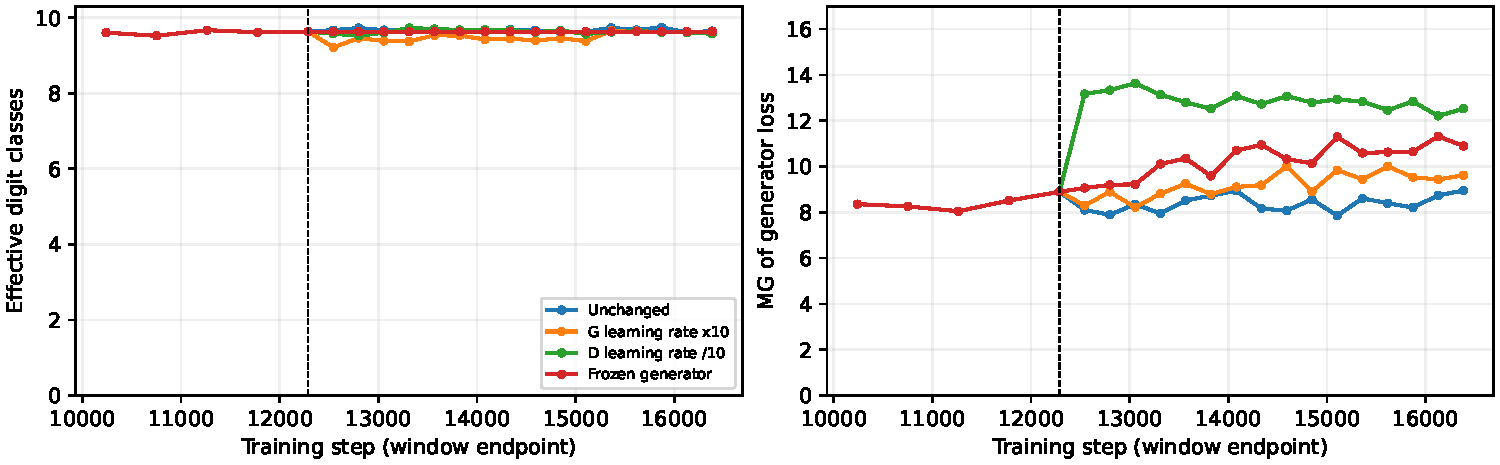
\includegraphics[width=\linewidth,height=.30\textheight,keepaspectratio]{mnist_branches/diagnostic.pdf}\end{center}

\newpage

\section*{5. Что показывает контроль с замороженным генератором}

После заморозки побитово совпадают все веса и статистики BatchNorm генератора. Проверены также точное совпадение выходных изображений на тестовых латентных векторах и одинаковые предсказания классификатора на всех сохранённых этапах. Поэтому изменение распределения изображений здесь исключено конструкцией опыта, а не только неизменной округлённой метрикой.

Тем не менее MG L\_G вырос с 8.36 до 10.65, примерно на 27\%. Средний loss также вырос: с 0.79 до 1.30. Причина различия объектов наблюдения проста: $L_G$ зависит не только от G, но и от обучающегося D. Следовательно, даже дешёвый и воспроизводимый отклик MG этого loss не является сам по себе свидетельством изменения разнообразия G.

Ветка с замедленным D дала рост MG примерно на 53\%, хотя итоговое разнообразие почти сохранилось. У ускоренного G рост около 14\%; у обычного продолжения менее 1\%. MG L\_D изменяется намного слабее: примерно \ensuremath{-}3\%, +4\%, +4\% и 0\% в соответствующих ветках. Выбор удачно выглядящего канала после анализа не проводился.

\section*{6. Устойчивость, суррогаты и границы интерпретации}

Позднее отношение MG(E=40)/MG(E=20) равно 1.42--1.52. Это не даёт оснований считать значения 8--13 точно восстановленным числом компонент. Вырожденных окон основного анализа не было. Дополнительные настройки меняют величину и иногда направление эффекта: например, в замороженной ветке при W=512, τ=4 оценка меняется с 12.22 до 10.81, хотя при основном τ=1 растёт. Поэтому настройка задержки по желаемому направлению недопустима.

Масштабирование того же лога в 10 раз не меняет MG. Сглаживание лога окном 8 способно заметно изменить оценку при неизменной модели: в конце ветки с замедленным D MG меняется с 12.53 до 6.94. В трёх IAAFT-суррогатах на контрольное окно сохраняются значения и приближённо амплитудный спектр; отношение MG исходного к медиане суррогатного --- 0.95--1.01. На этих окнах не обнаружен существенный разрыв с данным суррогатным контролем. Это не доказательство линейности или отсутствия нелинейной динамики.

\textbf{Подтверждённого события collapse нет.} Сохраняются все десять классов, эффективное число после разветвления остаётся примерно 9.2--9.7. Поэтому здесь нельзя оценивать полноту обнаружения collapse, AUC детектора или преимущество по задержке тревоги. Отсутствие такого события не доказывает, что MG не сработает при настоящем collapse. Но положительного подтверждения для статьи этот опыт не даёт.

\section*{7. Время: быстрый расчёт ещё не означает полезный детектор}

Независимый benchmark: Intel i5-12500H, CPU, один фактически измеренный поток Torch и BLAS, пять последовательных повторов после прогрева. Для MG --- одно уже записанное окно из 512 loss, без дополнительного forward. Для контроля изображений учитываются и генерация, и классификация. Это стоимость разных видов диагностики на контрольном этапе, а не равенство их информативности.

\begin{center}\small
\begin{tabularx}{\linewidth}{>{\raggedright\arraybackslash}Xrr}
\toprule
Диагностика & Медиана пяти повторов \\
\midrule
MG, одно окно & 10.50 мс \\
MG + повтор при E=40 & 23.05 мс \\
Простые статистики loss & 0.28 мс \\
Генерация и распознавание 512 изображений & 131.08 мс \\
Генерация и распознавание 10 000 изображений & 2537.68 мс \\
\bottomrule\end{tabularx}\end{center}

MG действительно дешевле большой проверки изображений, но преимущество детектора без подтверждённого события и проверенной точности не установлено. Контроль по 512 изображениям в этом маленьком десятиклассовом опыте тоже видит все классы; он должен оставаться обязательным конкурентом. Внутренние времена обучения и исходных оценок в логах получены с другим состоянием пула потоков, поэтому в сравнительную таблицу не подмешиваются.

\newpage

\section*{8. Вывод и воспроизводимость}

\textbf{В статью как положительный GAN-пример пока не добавлять.} На Stacked MNIST не пройден порог качества, на обычном MNIST не возник нужный переход. Проверка замороженного G показывает, что loss игры G/D может менять MG без изменения изображений. Это аргумент аккуратно выбирать наблюдаемую величину, а не объявлять провал MG для всех генеративных моделей.

Следующий научно оправданный шаг для этой идеи --- сначала получить качественный генератор и независимо воспроизводимую потерю разнообразия в устойчивой стандартной постановке, а затем проверять зафиксированный наблюдатель на новых seeds. Новый GPU-запуск сам по себе не устраняет отсутствие связи между выбранным loss и разнообразием. CIFAR-10, пять независимых подтверждающих seeds и практическое преимущество обнаружения в этом пилоте \textbf{не проверялись}.

Файлы находятся в research\_gan\_collapse. PROTOCOL.md содержит исходные настройки и все исследовательские изменения до вычисления MG. model.py и run.py реализуют обучение; prepare.py обучает независимый распознаватель; branches.py воспроизводит четыре продолжения; analyze.py вычисляет MG, простые статистики, чувствительность и суррогаты. audit\_benchmark.py проверяет неизменность замороженного G и повторяет замеры. make\_report.py и build\_report.py собирают этот PDF.

В pilot/base сохранён Stacked MNIST. В mnist\_pilot/base и base\_long --- оба этапа одиночного MNIST. В mnist\_branches --- четыре ветки, summary.csv, mg\_windows.csv, sensitivity.csv, controls.csv, benchmark.csv, fresh\_latents.csv и audit.json. В каталогах запусков: logs.csv, reference.csv, веса, индивидуальные предсказания распознавателя и контактные листы изображений. Это один seed GAN с общей предысторией, не семь независимых экспериментов.

Компактный архив gan\_collapse\_pilot\_results.zip содержит отчёт, скрипты, копию ядра MG, все таблицы и визуализации, распознаватель и контрольные точки, нужные для воспроизведения веток. Полные промежуточные веса и скачанный MNIST остаются в рабочей папке; данные повторно загружаются prepare.py. README.md содержит точные команды и оговорки. Код выполнен на CPU; GPU-версия в этом запуске не проверялась.

Предметная основа выбора задачи: Lin et al., PacGAN: The power of two samples in generative adversarial networks, NeurIPS 2018. Результаты PacGAN не переносятся на нашу меньшую архитектуру; опубликованный benchmark здесь не воспроизведён. Все приведённые численные результаты получены локально в текущем пилоте. Исходная статья проекта и её PDF не изменялись.
\end{document}